%\chapter{Role-Based Interaction in Multi-LLM Systems}\label{chap:roleint}\label{chap:role}

\chapter{Role-Based Interaction in Multi-LLM Systems}\label{chap:roleint}\label{chap:role}

\begin{learningbox}
In this chapter you will learn how multiple LLM agents behave when they are assigned roles and made to interact in a group. Specifically, you will be able to:
\begin{itemize}[leftmargin=*, nosep]
    \item Distinguish {\em role-based} multi-agent interaction (this chapter) from {\em open-ended} emergent simulations (Chapter \ref{chap:emergent}).
    \item Describe how LLM agents behave in {\em game-theoretic} settings when they interact with one another, and relate this to single-agent strategic findings (Chapter \ref{chap:behavior}).
    \item Explain {\em role-based collaboration patterns} and identify the frameworks that implement them.
    % \item Describe how agents are coordinated in practice, distinguishing orchestrator--worker from peer-to-peer topologies, and name the protocols used to connect them.
    \item Critically assess when  multi-agent collaboration improves performance, when it does not, and what new failure modes and {\em safety risks} are introduced by multi-agent interaction. 
\end{itemize}
\end{learningbox}

\section{From Single-agent to Multi-agent}
The previous chapter studied individual LLMs and LLM-powered agents through a behavioral lens: how a single model reads a communicative, social, or moral situation, and acts in it. In this chapter we move from single- to multi-agent settings and examine what happens when several LLM-based agents are made to interact, for example as opponents in game-theoretic contests and as collaborators in teams. The unit of analysis shifts from the behavioral profile of single models to interaction patterns and collective outcomes that arise between models.

\subsection{Mulit-Agent Simulations: History and Present}
The use of artificial agents to study interaction has a long history in the computational social sciences \citep{epstein1996growing,macal_tutorial_2010}. Traditionally, populations of agents with basic perception, reasoning, and decision-making capacities interacted in a virtual or, in case of robot-based simulations, real, experimental environment \citep{steels1995self,shoham2008multiagent}. The purpose of such simulations is usually to bridge theoretical and experimental work, using artificial behavior as a test ground for hypotheses about human behavior in domains where real-world experiments are difficult or costly. 

Two obstacles have historically limited this line of investigation: difficulty in verifying if behavior is realistic, and the high computational cost of simulating agent societies. Advances in agentic LLMs and simulation infrastructure \citep{rutherford2024jaxmarl} are changing this situation. LLM-based agents communicate in natural language, can process rich background knowledge, and can be given differentiated personas, making simulated interactions more expressive and more directly comparable to human interaction. 

\subsection{Role-Based versus Emergent Interaction}
Multi-LLM studies can be categorized based on the amount of control the researchers take over the simulation. At one end, every agent is assigned a \emph{role} in the form of a persona, objective, and interaction protocol. The research question is usually how the agents behave within the assigned structure and how well the resulting system performs as a whole, compared to other assigned structures and roles. At the other end, agents are placed in an open-ended environment without prior role assignment, and the research question is what social structure \emph{emerges}: group dynamics, conventions, and norms. This chapter is concerned with the role-based end of the spectrum, Chapter~\ref{chap:emergent} discusses the emergent side. 

This distinction matters for methodological choices as well as for the interpretation of results. In role-based systems, roles and interaction protocols are design decisions or experimental variables. Behavior is evaluated and interpreted against the goals that a system was designed for. In emergent settings, the goals or tasks play a role  at the background (or are entirely absent). The analysis is more open-ended and exploratory, closer to ethnography than to benchmarking. However, as will become clear, the distinction is not absolute: role-based systems regularly display  behavior that was they were not designed for.

\subsection{Five Dimensions of Multi-Agent Collaboration} \label{fivedimensions}
As a structuring principle for this chapter, we adopt the categorization by \citet{tran2025multi} along five dimensions of LLM collaboration: 
\begin{enumerate}
    \item \emph{Actors}: the agents involved, and whether they are homogeneous (instances of one model) or heterogeneous (different models or capability profiles)
    \item \emph{Interaction types}: cooperation, competition, or mixtures of both (``coopetition")
    \item \emph{Structures}: how the agents are organized, e.g. peer-to-peer, centralized, or distributed
    \item \emph{Strategies}: how collaboration is elicited, e.g. through role assignment or through model-level mechanisms
    \item \emph{Coordination protocols}: the mechanisms that tie agents together and regulate their communication
\end{enumerate}
The systems discussed in this chapter make different choices along these five axes, and keeping these dimensions in mind makes it easier to see what is new about each framework.

\subsection{A Methodological Note}
Evaluating multi-agent systems inherits every methodological difficulty of evaluating single models: prompt sensitivity, possible leakage of test materials into training data, and sampling variability. Plus, it adds new difficulties of its own: 
\begin{itemize}
    \item Reported results are often harder to reproduce because small variations in one agent's output cascade through subsequent interaction, increasing run-to-run variability.
    \item It can be unclear what causes performance differences: the multi-agent collaboration itself, the coordination protocol, the embedded prompt engineering for the role distribution, or simply the additional inference budget multiple agents consume cumulatively.
    \item Construct validity shifts to the level of social-interactive terminology: concepts such as {\em team work}, {\em discussion}, or {\em collective decision-making} carry rich human connotations that the actual simulation may not warrant.
\end{itemize}
With these caveats in mind, the chapter proceeds to the simplest multi-agent setting: LLM agents facing each other in strategic settings, with no roles assigned beyond the game itself (Section \ref{sec:strat}). Next, we examine what changes when interaction is streamlined by defining coordination protocols and explicit roles (Section \ref{sec:roletask}).

\section{Strategic Interaction Among LLM Agents} \label{sec:strat}
In Chapter \ref{chap:behavior} we examined how LLMs behave when prompted to play economic games against a scripted opponent. Here we consider studies in which {\em LLM agents interact with one another} in game-theoretical scenarios. The agents in this section are symmetric peers: each pursues its own interests and none is assigned a coordinating or supervisory role. We look first at benchmarks that score LLM agents across many games at once, and then at behavior in single, richer simulation platforms built around one scenario.  

\subsection{Benchmarking Strategic Ability Across Games} 
The MAgIC study \citep{xu2024magic} uses social deduction games (Undercover and Chameleon) and game theoretic scenarios such as cost sharing, the multi-player Prisoner's dilemma, and public goods games. The goal is to extract seven capabilities: rationality, judgment, reasoning, deception, self-awareness, cooperation, and coordination, as shown in Figure~\ref{fig:radar}. LLMs in off-the-shelf and enhanced forms are evaluated on these capabilities in multi-agent settings.

GPT-o1 and GPT-4 score significantly better than the other models. LLMs generally score high on judgment, rationality and cooperation, some also on deception, but lower on reasoning and all but one score low on coordination. The exception is GPT-o1 enhanced with probabilistic graphical modeling, an implementation of a theory of mind-like competence inspired by \citet{kollerfriendman2009pgm}. The authors show that probabilistic graphical modeling boosts LLM performance across the board. This is consistent with the general evidence discussed in Section~\ref{sec:theoryofmind} that humans lean heavily on theory of mind in strategic settings.

\begin{figure}
  \begin{center}
    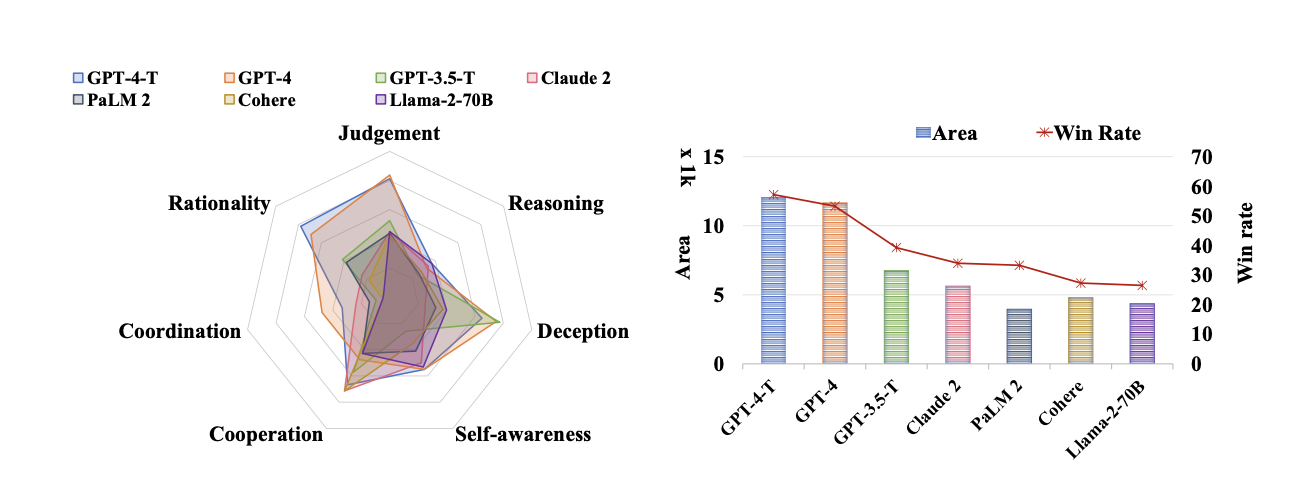
\includegraphics[width=\textwidth]{figures/radar}
    \caption{LLM's Performance on various Metrics \citep{xu2024magic}}\label{fig:radar}
  \end{center}
\end{figure}

A benchmark that isolates coordination as the object of study, rather than as one trait among several, is the LLM-Coordination Benchmark \citep{agashe2025llm}. LLMs are evaluated on two distinct tasks: agentic coordination in pure cooperation games and question answering about those games (see Figure \ref{fig:agashe}). The experiments find that LLM agents perform well as long as decision-making can rely on environmental variables, but poorly when success requires actively reasoning about a partner's beliefs and intentions. Concretely, such environmental variables include elements such as the game layout, locations of objects, where each agent is currently positioned, which doors are open, and so on. The clearest illustration is Overcooked-AI, the game where LLMs did best. This game is fully observable, and its action space consists of moves such as {\em pick up an onion from onion dispenser 1} and {\em place onion on plate 0}. Under most scenarios and layouts, LLMs only need to consider the next best steps based on the state of the game environment, without taking into account other agent's perspectives.

This asymmetry becomes especially clear when comparing performance on Overcooked with scores in Hanabi, a game in which every action requires reasoning about the partner's beliefs. On Overcooked, zero-shot LLM agents can match or outperform specially trained reinforcement learning baseline models. On Hanabi, however, the reinforcement learning baselines show near-perfect scores, whereas most LLM agents barely score at all. The best LLM agent (based on GPT-4-turbo) reaches only about half the maximum score, even when enhanced with explicit theory of mind reasoning and self-verification steps. Without such enhancements, the scores of strong models such as  GPT-4-turbo collapses almost entirely, indicating that the measured ability is partly a feature of the agent framework rather than the model alone. The LLM agents did prove more robust in cross-play: reinforcement learning methods degrade sharply when playing unseen partners, whereas the zero-shot nature of LLM agents facilitates transfer to unseen partners without performance loss.

The question-answering component of the study (see Figure \ref{fig:agashe}, right column) breaks the problem down by targeting environment comprehension, ToM, and joint planning, separately. They find that LLMs score generally high on the first category (>80\% for the best model), lower on ToM, and worst on joint planning (<40\% for the best model, below random chance for open-source models). This is consistent with the observed difference in scores between Overcooked (environment-driven) and Hanabi (ToM- and planning-driven).

\begin{figure}
  \begin{center}
    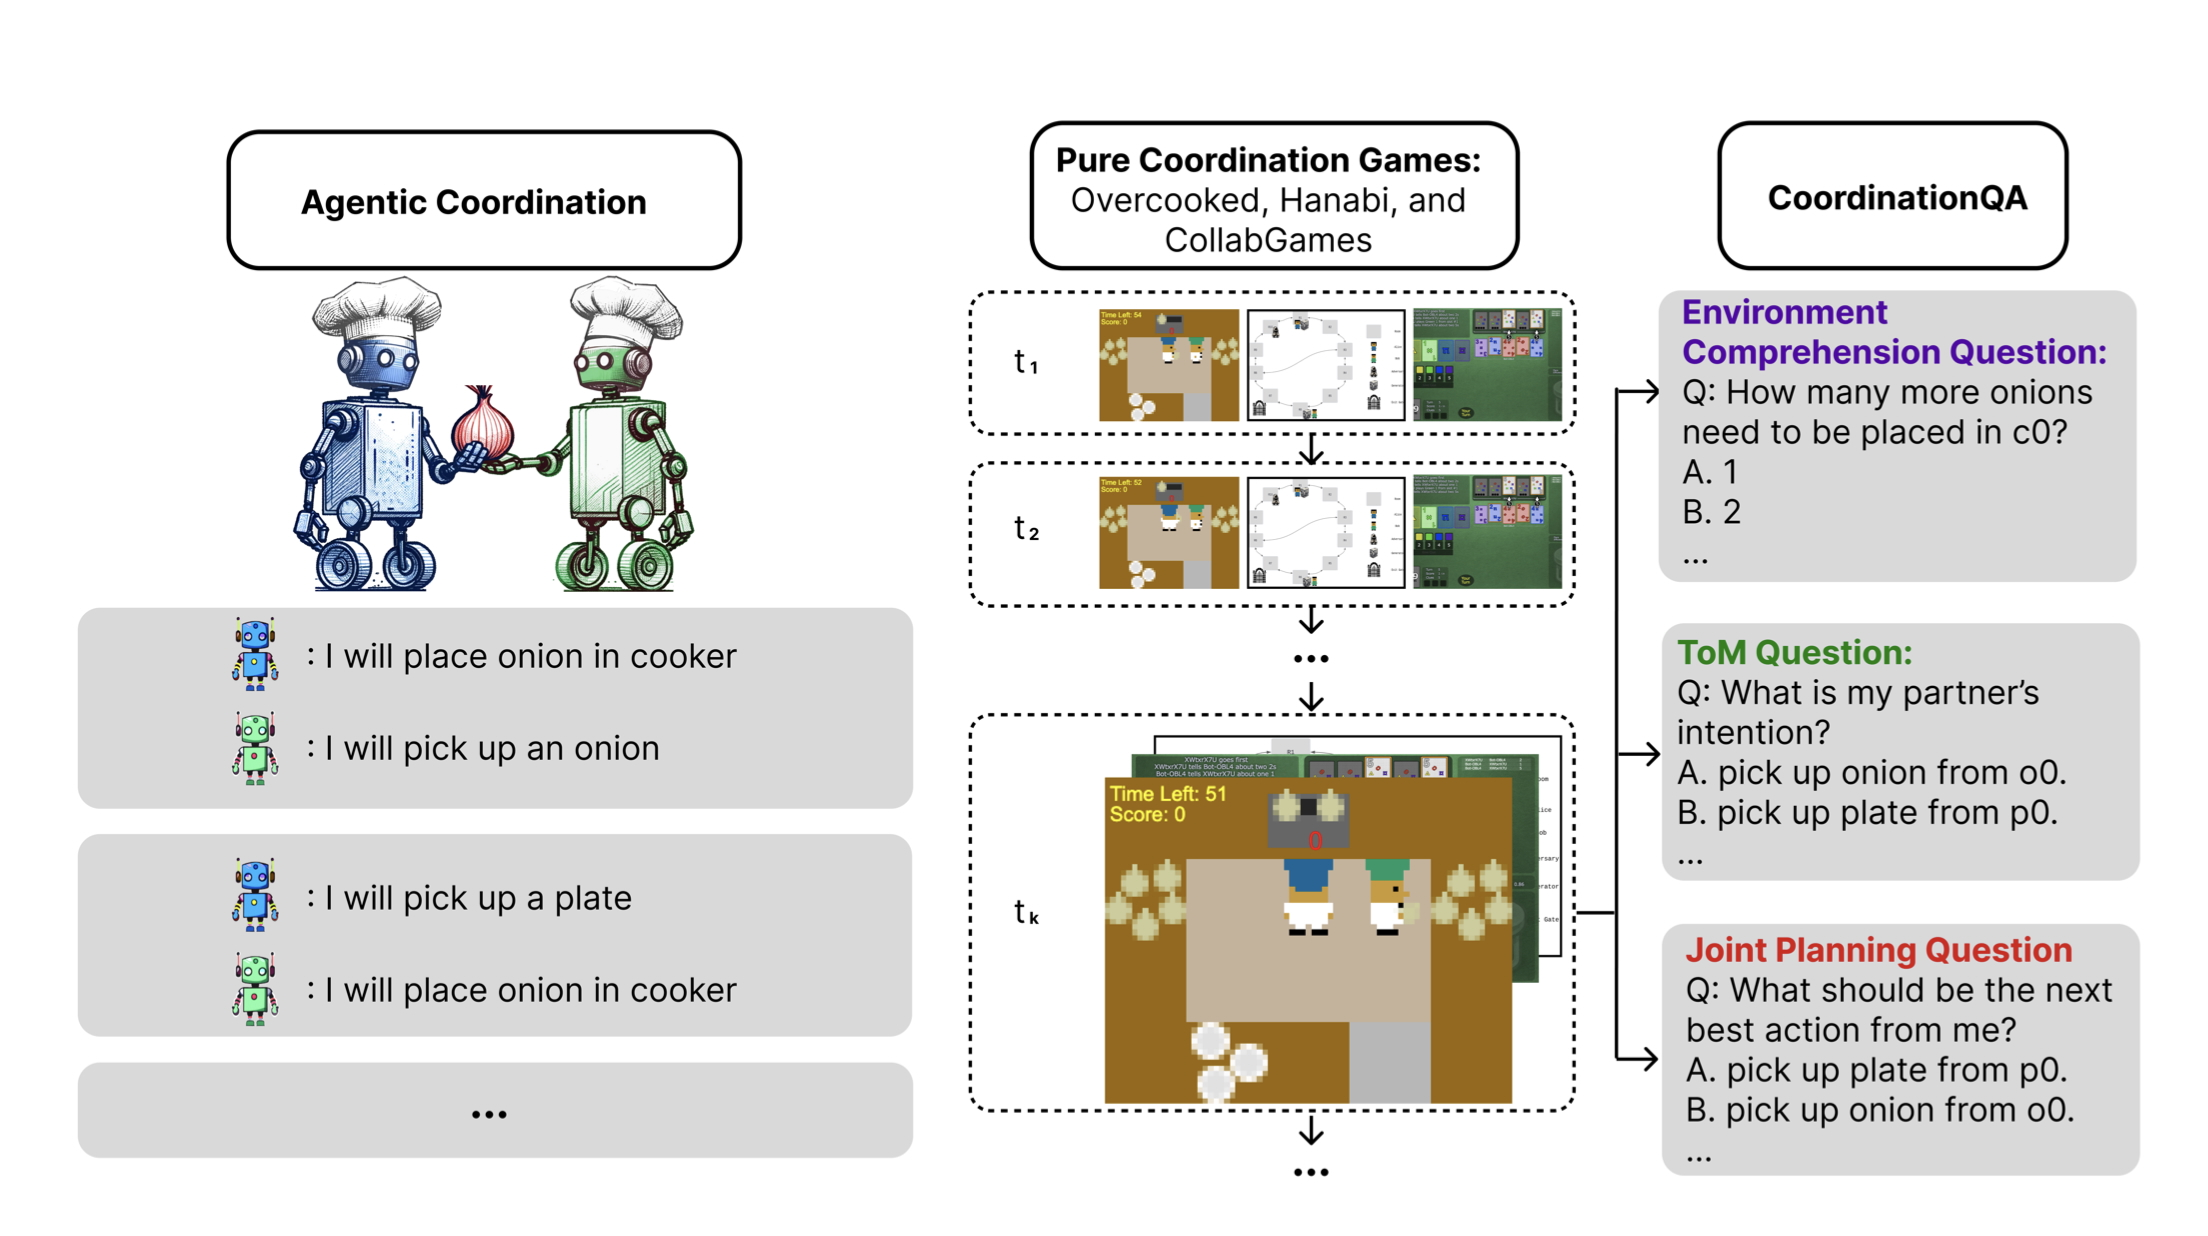
\includegraphics[width=14cm]{figures/llmcoordinationbank} 
    \caption{Illustration from the LLM Coordination Benchmark \citep{agashe2025llm}, which uses two types of measures to assess agentic coordination: behavior in pure coordination games in which agents must cooperate to maximize gains (middle) and detailed questions about those games (right)}\label{fig:agashe}
  \end{center}
\end{figure}

The key characteristic of pure cooperation games is that agents must fully cooperate with each other with no competitive incentives. In contrast, in competitive settings such as the Prisoner's Dilemma (or the mixed-motive games in benchmarks like MAgIC), an agent faces a genuine tension between individual and collective payoff. In such games, when an LLM fails to cooperate, the reason is unclear. The agent may be bad at coordination \textit{or} it might reason strategically about individual gains. In pure cooperation games, there is never any reason to defect, so any failure to cooperate is a genuine lack of coordination ability.

\subsection{Strategic Interaction in Single-Scenario Platforms}
Benchmarks aggregate over many small games. A complementary line of research builds single scenarios and studies agent behavior in-depth. 

Alympics \citep{mao2023alympics} provides a controlled playground for simulating strategic interaction among LLM-driven agents, illustrated by a multi-round water-allocation challenge in which scarce survival resources must be distributed over time, see Figure~\ref{fig:water}.
\begin{figure}
  \begin{center}
    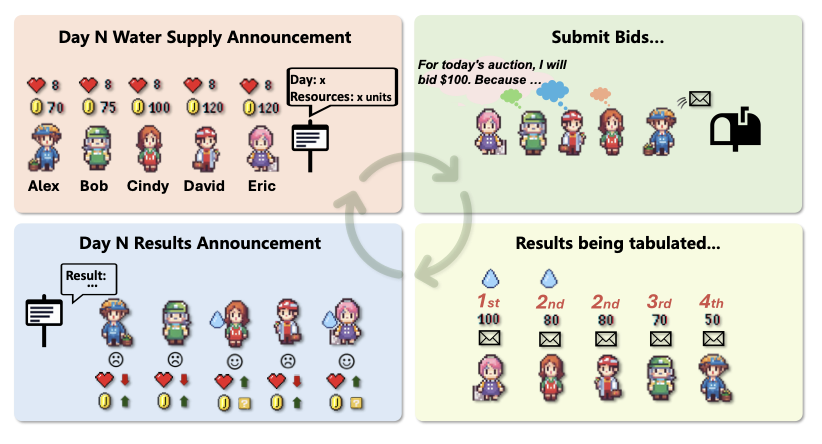
\includegraphics[width=13cm]{figures/water}
    \caption{Alympics Water Allocation 
    Challenge Game \citep{mao2023alympics}}\label{fig:water}
  \end{center}
\end{figure}

AucArena \citep{chen2023put} simulates auctions, across LLaMa 2.13b, Mistral 7b, Mixtral 8x7b, Gemini 1.0, and GPT 3.5/4.0, finding that the most capable LLMs such as GPT-4 possess skills for auction participation such as budget management and goal-focus, though performance varies even for that model, and the authors point to considerable room for improvement.

\subsection{Conclusion}
Across benchmarks and single-scenario platforms alike, coordination emerges as the consistent weak spot of LLM agents. Stronger LLMs score well on rationality and judgment in MAgIC, manage budgets sensibly in AucArena, and match trained RL agents in environment-driven cooperation. However, all but the strongest and most heavily scaffolded models fail when success requires reasoning about what a partner believes and intends. 

In other words, models fail to consistently \emph{integrate} theory of mind reasoning with their behavior. In Chapter \ref{chap:behavior}, failures of this kind were referred to as the knowing-doing or literal-functional gap: GPT-4 could respond accurately when prompted to predict the alternating pattern in Bach or Stravinsky, but failed to enact it when playing. However, the multi-agent studies reviewed here complicate that diagnosis. In the question-asking section of the LLM Coordination Benchmark, the questions about joint planning pose exactly the decision the agent faces at each step of the game play. It is on these questions that the models perform worst (and on ToM questions not much better). Question-answering scores correlate positively with agentic performance across games. In other words, knowing and doing move together here: where models act poorly, they also reason poorly when the action problem is posed to them directly. For pure coordination tasks, the deficit thus lies in taking the partner's perspective (ToM) and joint planning itself, rather tan in translating reasoning into action.

On a different level, the knowing-doing gap  reappears. In Hanabi, GPT-4-turbo  reaches reasonable performance only when scaffolded with explicit ToM reasoning and self-verification steps. Without these in place, it commits fatal errors in every Hanabi trial. In other words, it acts wrongly initially, but recognizes and corrects these errors when prompted to check  the reasoning and verification steps. Similar performance boosts were caused by probabilistic graphical modeling in MAgIC and Social Chain-of-Thought in strategic-behavior studies discussed in Chapter \ref{chap:behavior}. The boundary between \emph{LLMs cannot reason about others} and \emph{LLMs do not spontaneously deploy such reasoning} is apparently thin, and agentic embedding in the form of structured reasoning and verification steps can bring out the latter. 

The next section examines a different, complementary response to the same problem: instead of upgrading the agents' reasoning, one can structure the interaction itself, by assigning roles.

\section{Role-Based Task Solving and Teamwork}\label{sec:roletask}
In the previous section, agents were symmetric peers and coordination had to emerge from their own strategic reasoning (with limited success). In the studies discussed in this section, coordination is designed-in using interaction protocols and assigning roles with distinct objectives. 

In terms of the five dimensions defined in Section \ref{fivedimensions}, the studies vary the \emph{strategies} and \emph{structures} while keeping the overall interaction type cooperative. We proceed from the simplest to the most complex structure: complementary pairs, multi-party debate, teams, and social role-play under pressure.

\subsection{Complementary Pairs}
LLMs can perform tasks in pairs where they are assigned complementary roles, such as creator-critic or manager-worker. In these pair-wise setups, each LLM agent is given a distinct role and objective, and they communicate to jointly solve tasks. 

In the CAMEL framework (Communicative Agents for ``Mind" Exploration) \citep{li2023camel}, two LLMs have predefined roles to perform, to work on a goal such as a coding task (See Figure \ref{fig:camel}). Through cooperation, together they drive a conversation without explicit continuous human prompting. CAMEL uses inception prompting and role descriptions so that  agents stay in character and collaborate towards the goal. The agents are prompted to  break down complex problems in manageable steps through their dialogue. During each interaction step the LLM agents effectively generate their own inference-time training data, making the cognitive process visible for human inspection,  while at the same time enhancing autonomous task performance.

\begin{figure}
  \begin{center}
    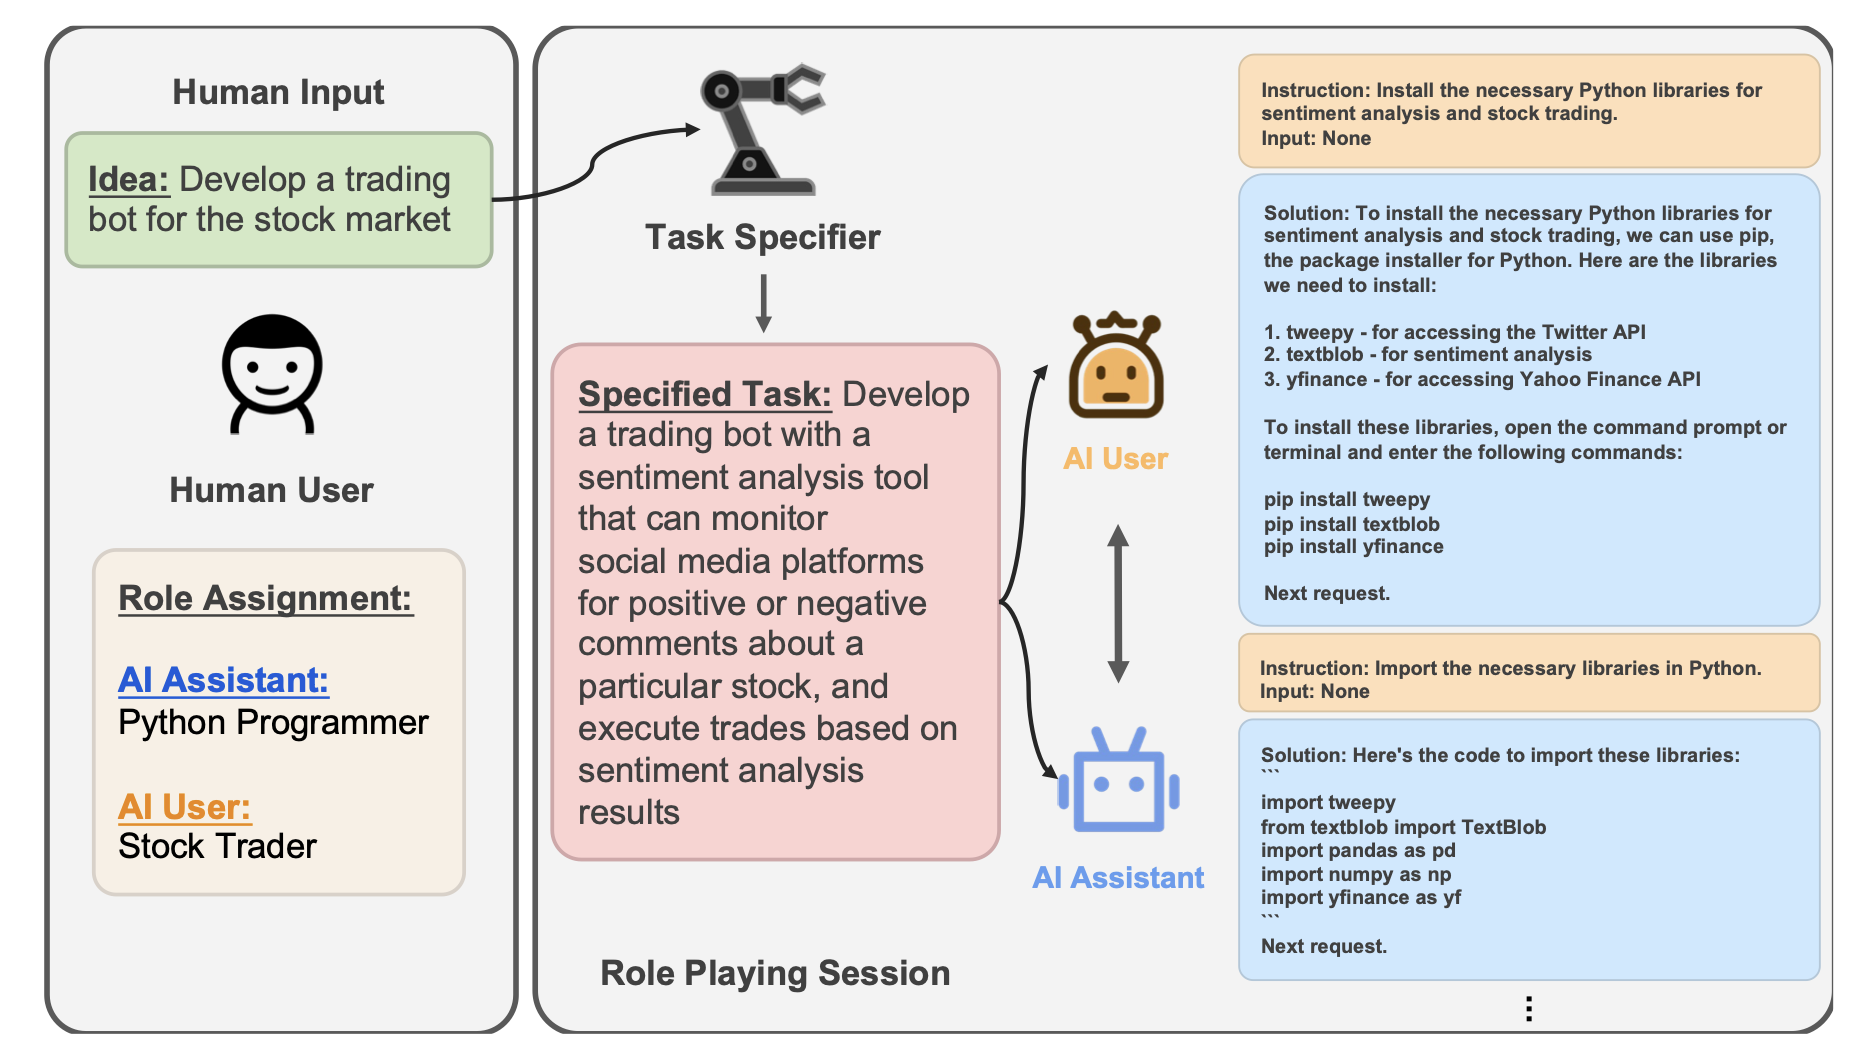
\includegraphics[width=\textwidth]{figures/CAMEL}
    \caption{Role-playing in CAMEL \citep{li2023camel}}\label{fig:camel} 
  \end{center}
\end{figure}

Other studies have paired an LLM creator (or generator) with an LLM judge (or critic) in a self-reflective setting. In this way the generative power of LLMs is leveraged through one agent, while adherence to rules or quality guidelines is enforced by the other. Constitutional AI \citep{bai2022constitutional} employs one LLM to critique another LLM’s responses against a set of ethical or quality guidelines, suggesting revisions. The authors show that this kind of two-agent feedback yields refined final outputs that are aligned with the desired principles.

A third form of pair-wise interaction follows human tutoring dynamics: teacher-learner or expert-novice. Chapter~\ref{sec:distillation} discusses various examples of this structure in the context of distillation.

All three pairings exploit the same idea: one agent's oversight can correct the other's mistakes, leading to more robust joint performance than either agent achieves alone.

\subsection{Debate and Discussion}
Beyond pairs, a prominent example of role-based interaction is the use of debate and discussion between LLMs to improve reasoning and task performance.

\citet{du2024debate} demonstrated that when multiple LLM instances propose answers and critique each other’s reasoning through several rounds of debate, they can reach a more accurate consensus answer with higher factual correctness. This approach, described in terms of Minsky's society of minds \citep{minsky1988society}, significantly reduced reasoning errors and hallucinations in tasks such as math word problems and factual question answering.

\citet{liang-etal-2024-encouraging} propose a multi-agent debate (MAD) setup where two LLM agents take opposing sides in, for instance, a tit-for-tat negotiation (see Section \ref{sec:strategic}) while a third agent acts as a judge. The role of the judge is to guide the discussion towards a final solution. The structured debate encourages divergent thinking and can push a weaker model enhanced with MAD (such as GPT-3.5) to outperform a stronger model without MAD (such as GPT-4) on a challenging benchmark. The authors discuss how their MAD setup overcomes a known problem in model scaffolding with self-reflective steps. Self-reflection can induce so-called \emph{degeneration of thought}: once a model gains confidence in a certain solution direction, self-reflection can reinforce the confidence even if the direction is wrong. In the MAD debating-setup, the other agent can push towards a different direction direction to avoid thought degeneration.

ChatEval applies this debate pattern to text evaluation \citep{chan2023chateval}. Noting that the quality of human text assessment improves when multiple annotators collaborate, the authors create a multi-agent referee team with debater agents, diverse role specifications, and different communication strategies (see Figure \ref{fig:chateval}), moving beyond single-agent prompting strategies.

\begin{figure}
  \begin{center}
    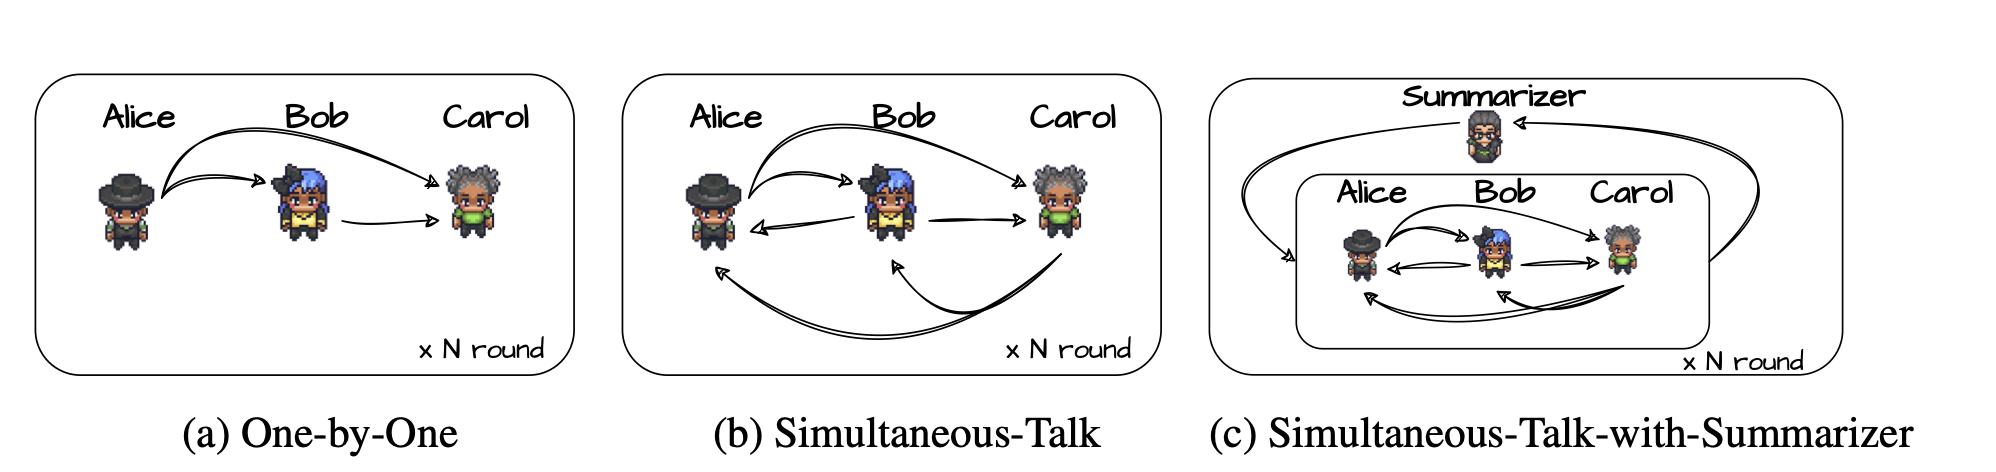
\includegraphics[width=14cm]{figures/chateval}
    \caption{Three Different  Communication Strategies in ChatEval \citep{chan2023chateval}}\label{fig:chateval} 
  \end{center}
\end{figure}

Another approach, also motivated by Minsky's society of minds, is ReConcile,  a multi-agent framework designed as a round table conference among diverse LLM agents \citep{chen2023reconcile}. The framework enhances collaborative reasoning between LLM agents via multiple rounds of discussion. The agents must try to convince one another to improve their answers. Experiments on seven benchmarks demonstrate that a confidence-weighted voting mechanism significantly improves LLMs’ reasoning. Furthermore, the authors find that diversity (using different underlying models) is critical for performance. 

MindStorms introduces an LLM-based implementation \citep{zhuge2023mindstorms} on the CAMEL framework \citep{li2023camel}. Extensive experiments are reported with up to 129 agents solving common AI problems: visual question answering, image captioning, text-to-image synthesis, 3D generation, egocentric retrieval, embodied AI, and general language-based task solving. The authors find that, in specific applications, mindstorms among many members outperform those among fewer members, and longer mindstorms outperform shorter ones.

\subsection{Role-Based Software Teams}
An interesting application of role-based collaboration is software development, where  simulated  teams that are entirely staffed with LLM agents develop software.

Automated programming by LLMs has suffered from problems, such as logic inconsistencies and hallucinations that cascade throughout a development pipeline. MetaGPT \citep{hong2024metagpt} builds on workflows that have proven to be effective in human software teams. The framework converts Standard Operation Protocols (SOPs) into prompt sequences and assigns agents the roles of a software company: product manager, architect, engineer, QA tester. In this way, the agents pass structured intermediate artifacts down an assembly line. The product manager makes a requirements document, the architect turns this into a design, the engineers code. In this way, complex tasks are divided into  manageable subtasks and agents can verify the process step-by-step, significantly reducing errors.

Similarly, \citet{qian-etal-2024-chatdev} have introduced ChatDev, a virtual software company in which agents collaborate through the phases of a development process: design, coding, and testing. Collaboration is organized as a \emph{chat chain}: each phase is decomposed into short conversations between an instructor and an assistant agent (see Figure \ref{fig:chatdev2}). Using a communication protocol that makes agents ask for more details before responding, leads to what the authors call \emph{dehallucination}, increasing the reliability of each step. The framework demonstrates how structured communication in natural language can facilitate multi-agent collaboration.

\begin{figure}
  \begin{center}
    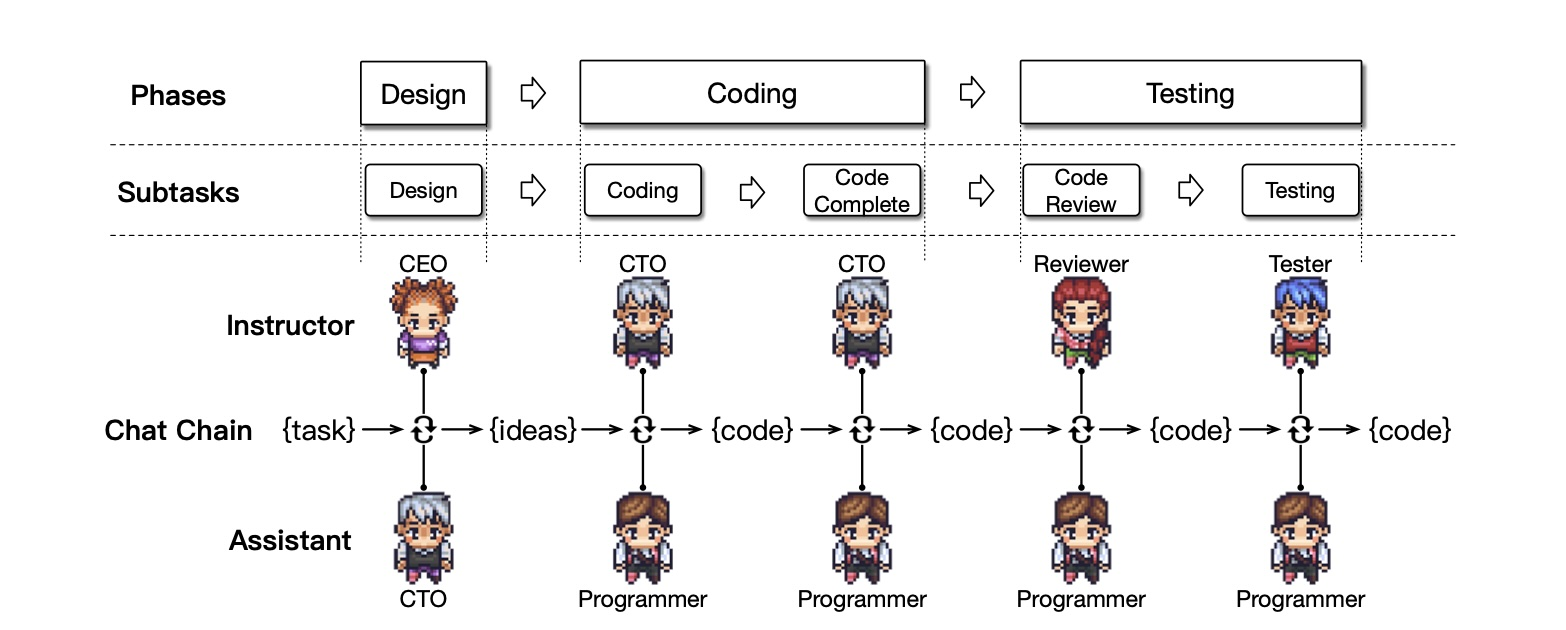
\includegraphics[width=14cm]{figures/chatdev2.jpg}
    \caption{The Chain-Structured Workflow in ChatDev \citep{qian-etal-2024-chatdev} based on Multi-Turn Dyadic Communication between Agents Powered by ChatGPT-3.5}\label{fig:chatdev2} 
  \end{center}
\end{figure}

Where MetaGPT and ChatDev hard-wire a particular organization structure, AutoGen \citep{wu2024autogen} provides a flexible programming framework based on conversations between customizable agents that can combine LLMs, tools, and human input. It was designed as an open-source platform that enables developers to define agents and interaction structures depending on the application. Experiments demonstrate effectiveness in tasks across mathematics, coding, question-answering, entertainment, and other domains.

\subsection{Social Role-Play}
The systems discussed above assign roles to solve tasks. A final line of work assigns roles in order to study social behavior itself: what do LLM agents do when placed in socially demanding or conflicting situations?

\begin{figure}
  \begin{center}
    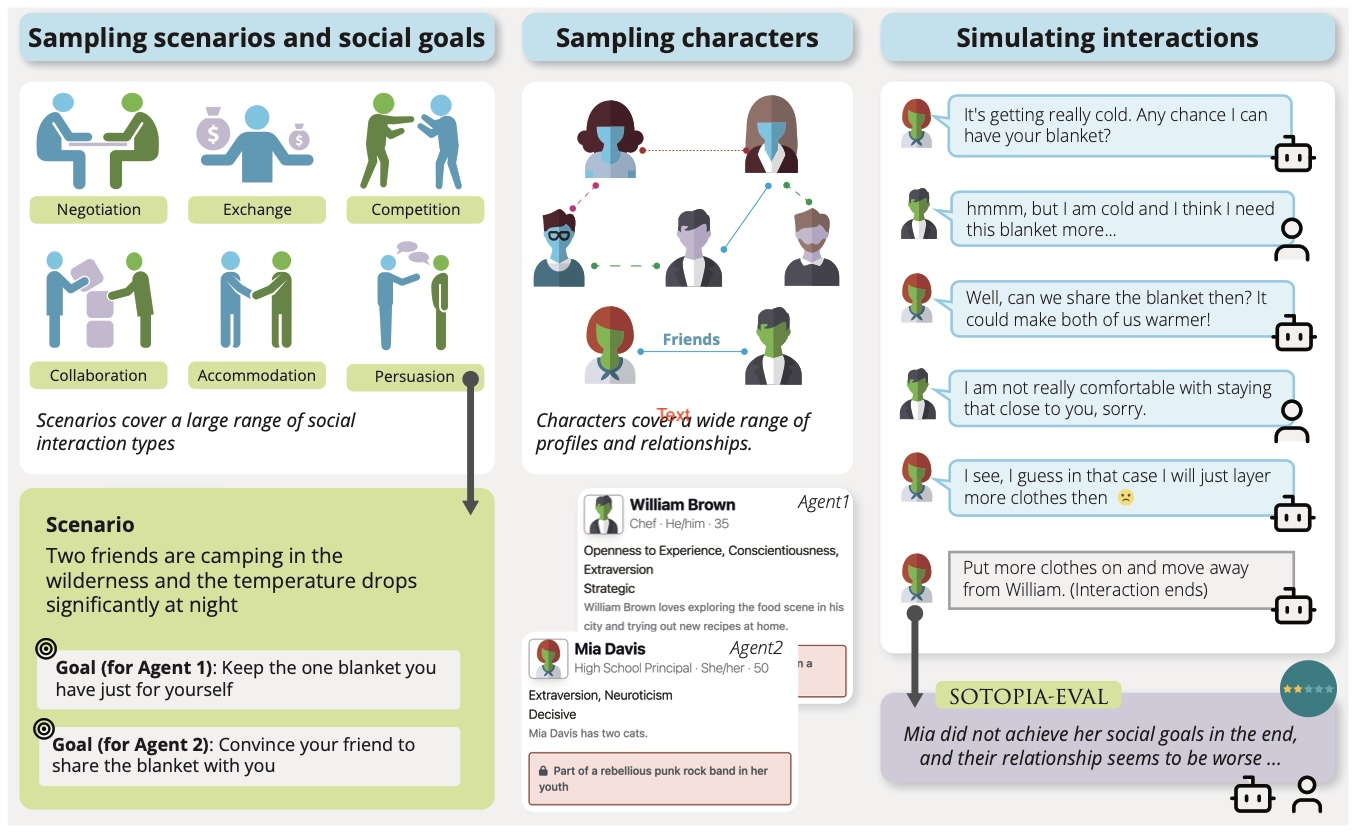
\includegraphics[width=14cm]{figures/sotopia.jpg}
    \caption{Illustration of a Scenario with a Conflicting Social Goal from SOTOPIA \citep{zhou2023sotopia}}\label{fig:sotopia} 
  \end{center}
\end{figure}

In SOTOPIA \citep{zhou2023sotopia} agents coordinate, collaborate, and compete to achieve complex social goals. The SOTOPIA environment features a large and diverse task space by sampling \emph{interaction episodes} from 90 (automatically generated) social scenarios with 40 characters with individual personalities, occupations, secrets, background stories, and relationships with other characters (Figure~\ref{fig:sotopia}). The authors evaluate the social intelligence of agents based on different LLMs against that of human participants, observing various trends:
\begin{itemize}
    \item Models that perform well on static benchmarks involving social reasoning (such as ToMBench, see Section \ref{sec:theoryofmind}) do not necessarily succeed in interactive scenarios, illustrating the knowing-doing gap once again (Section~\ref{sec:strategic}.
    \item Weaker agents weaken their conversation partners, which is  the reverse effect of the conversational advantages  discussed above, where agents prevented each other from thought generation and other errors.
    \item Divulging secrets and violating social norms is observed across all models, consistent with observations discussed in the context of moral behavior (Section \ref{sec:moral}).\
    \item Humans perform significantly better on the most challenging SOTOPIA tasks compared to even the best performing model (GPT-4).
\end{itemize}
The authors argue that the dynamic and interactive nature of SOTOPIA poses unique challenges for LLM agents that static benchmarks systematically fail to reveal.

Social interaction in an extreme setting was studied in \citep{campedelli2024want}. Inspired by the infamous Stanford Prison experiment \citep{zimbardo1972stanford}, the authors examine the emergence of persuasive and abusive behavior in a setting of prisoners versus prison guards. It was found that the assigned personality of prisoner and guard impact both persuasiveness and the emergence of anti-social behavior. Crucially, this demonstrates that anti-social behavior can emerge in LLM agents through role assignment and a specific interaction environment. This reveals a striking parallel to the original experiment with human participants, and reminds us once again of the gap between how a model judges situations (generally reflecting population-average moral norms) and how an agent can behave once it is employed in a specific context of action (see also Section \ref{sec:moral}). This study  also finds that role assignment is not a neutral engineering instrument: it can shape behavior in untoward ways.

To simulate strategic decision-making in cooperative settings, researchers have introduced GovSim \citep{piatti2024cooperate}. They study how ethical considerations, strategic planning, and negotiation skills impact cooperative outcomes. Most LLMs fail to achieve an equilibrium since they fail to understand the long-term effects of their actions on the group. Interestingly, the introduction of a special \emph{universalization} reasoning language \citep{levine2020logic} (prompting models to ask the Kantian question: \emph{What if everybody does that?}) allowed more models to achieve a sustainable outcome. Related results were demonstrated in NegotiationArena, introduced by \citet{bianchi2024well}. They showed how LLM agents can conduct complex negotiations through flexible dialogue in negotiation settings. The flexible dialogues significantly improved negotiation outcomes by employing different behavioral strategies. 

\subsection{Conclusion}
The studies in this section respond to the coordination weaknesses identified in Section \ref{sec:strategic} not by making individual agents better reasoners (as in \ref{sec:enhancement}), but by structuring the interaction around them. Complementary roles tell each agent what its contribution should be, while interaction protocols and SOPs regulate when and in what form agents communicate. In some setups, a judge or voting mechanism can help to channel disagreement to a productive resolution.

Roles and interaction protocols provide crucial scaffolding where internal coordination would otherwise fall short. This can be seen as a multi-agent analogue of the structured reasoning schemes discussed in Chapter \ref{chap:behavior}, such as Social Chain-of-Thought, probabilistic graphs, or deliberation around moral rules. Such schemes turned out to boost performance where unconstrained reasoning did not. In both the single- and multi-agent cases, the model's latent (social, moral, etc.) knowledge and behavior are real, but need to be activated through an explicit structure.

% Related to debate and discussion setups, researchers have explored teacher-learner dynamics with LLMs, where an expert LLM provides hints or feedback to a less capable LLM, mirroring human tutoring \citep{zhou2023sotopia}. These role-alignments leverage the same idea as the MAD setup: one agent’s oversight can correct the other’s mistakes, leading to more robust performance and a lower chance of falling into thought-degeneration loop holes. 
%AutoGen \citep{wu2023autogen} is designed to facilitate the development of multi agent LLM applications that span a broad spectrum of domains and complexities. The programming paradigm is centered around agent-agent conversations. Experiments demonstrate the effectiveness of the framework in  example applications ranging from mathematics, coding, question answering, operations research, online decision-making, to entertainment.

% Sotopia is another role-playing environment for multi-agent interaction \citep{zhou2023sotopia}. In Sotopia, agents coordinate, collaborate, exchange, and compete with each other to achieve complex social goals. In experiments with LLM-agents and humans,  GPT-4 achieves a significantly lower goal completion rate than humans and struggles to exhibit social commonsense reasoning and strategic communication skills. The contrast between GPT-4's lower performance in Sotopia and good performance on other metrics of social reasoning (see Section \ref{sec:tom}) is most likely explained by Sotopia's focus on strategizing and goal-directedness, aspects on which GPT-4 has been reported to score lower \citep{hou2024entering}.

\section{Concluding Remarks}
This chapter moved from LLM agents facing one another in strategic games, through role-based collaboration patterns and the multiple setups that coordinate them in practice, to a critical assessment of when multi-agent systems work or fail. 

In Chapter \ref{chap:behavior} we found single models that coordinate poorly and that can formally predict what a partner will do without acting on that prediction in an agentic implementation. Both these patterns transfer to the multi-agent setting. Across benchmarks and platforms (e.g. \citep{xu2024magic, agashe2025llm}), interacting LLM agents could reason about self-interest, yet failed to coordinate their behavior such that they could turn this reasoning into a strategic advantage. A dominant issue is their ability to condition their behavior on their partners' perspective, a problem foreshadowed in the gap between knowing-doing or literal-functional competence for theory of mind, discussed in Section~\ref{sec:theoryofmind}. This resonates with work that systematically identifies inter-agent misalignment as a dominant failure category for multi-agent systems \citep{cemri2025masfail}.

This literal-functional problem, once again, links to construct validity: just as acing a theory of mind test does not establish a human-grade capacity for social reasoning, a multi-agent setup outperforming a single LLM query does not establish collective intelligence. Strong baselines, matched inference budgets, and ablations of the collaborative structure and interaction protocols would be the mulit-agent equivalents of the perturbed ToM testing discussed in Section \ref{sec:theoryofmind}. More research is needed in the multi-agent field to establish a solid empirical picture of where agentic LLM interaction stands.

Finally, the multi-agent setting adds new risk categories. Role-assignment turned out to be capable of activating anti-social and even abusive behavior in a setting inspired by the Stanford Prison Experiment \citep{campedelli2024want}. In other studies, miscoordination, cascading hallucinations, and mutual reinforcement of weaknesses, triggered norm violations, divulging of secrets, and reduction of task performance. Where specifying roles and interaction protocols scaffolded behavior and boosted performance in some cases, in other cases these were a hindrance or a source of risk. 

In the next chapter we discuss studies in which roles and protocols are not assigned, but emerge from the interaction itself.


\bibliographystyle{plainnat}
\bibliography{agenticbook,refs,case,synthetic}
